\documentclass[pdftex,11pt,a4paper]{article} 
% margin size
\usepackage[margin=1in]{geometry}

% Math and algorithms
\usepackage{amsmath,amssymb,amsthm,esint}  % For both in-line and equation mode
\usepackage{bbm}
\usepackage{mathdots}
\usepackage{bm}
\usepackage{algorithm}
\usepackage{algorithmic} % Algorithm styles, need to be nested for the example shown
\usepackage{aliascnt}
\numberwithin{equation}{section} % Numbering of our equations per section
\newtheorem{theorem}{Theorem}
\newtheorem{definition}{Definition}
\newtheorem{proposition}{Proposition}
\newtheorem{corollary}{Corollary}
\newtheorem{remark}{Remark}

\usepackage{setspace} %Spacing on the front page for crest and titles
\usepackage[]{fncychap} % Styles can be Sonny, Lenny, Glenn, Conny, Rejne, Bjarne and Bjornstrup
\usepackage[hyphens]{url} % Deals with hyphens in urls to make them clickable
\usepackage{xcolor} % Great if you want coloured text

% Figures
\usepackage{wrapfig}
\usepackage{graphicx} % Inserting images
\graphicspath{ {figures/} } 
\usepackage{caption}
\usepackage{float}

% Tables
\usepackage{tabularx}
\usepackage{multirow} 
\renewcommand{\arraystretch}{1.5}

% Appendix
\usepackage{appendix} 

\usepackage{natbib}
\usepackage{comment}
\usepackage{booktabs}

% purple placeholders for paragraphs still to be written
\newcommand{\ph}[1]{\textcolor{purple}{[#1]}}

% Tikz figures
\usepackage{tikz}
\newcommand{\ImageWidth}{14cm} 
\usetikzlibrary{decorations.pathreplacing,positioning, arrows.meta} 

% Fancy headers and footnotes
\usepackage{fancyhdr}
\usepackage[symbol]{footmisc}
\renewcommand{\thefootnote}{\fnsymbol{footnote}} 

% Hyperlinks and auto-references
\usepackage[hidelinks]{hyperref}  
\def\sectionautorefname{Section}
\def\appendixname{Appendix}
\newcommand{\propositionautorefname}{Proposition}
\newcommand{\definitionautorefname}{Definition}
\newcommand{\corollaryautorefname}{Corollary}  

\setlength{\footnotesep}{0.5cm}
%%%%%%%%%%%%%%%%%%%%%%%%%% DOCUMENT STARTS %%%%%%%%%%%%%%%%%%%%%%%%%%%%% 

\begin{document} 
% Front page 
\pagestyle{empty}

% Logo, Title
\begin{center}
	\begin{figure}
		\centering
		
\includegraphics[scale=0.8]{tec_logo.png}
		\vspace{10mm}
	\end{figure}
	\textbf{\begin{huge}
		Algorithmic Analysis of SARS-CoV-2 Sequences \\
	\end{huge}} 
	\vspace{10mm}
\end{center}

% Subject, Code and Date
\begin{center}
	\vspace{5mm}
	\textbf{\large Advanced Algorithms Design}\\ 
    %\vspace{2mm}
    {\large TC2038, Situation Problem 1\\} 
	%{\large January 2023\\}
	\vspace{5mm}
	\textbf{\large Santiago Hernández\\}
	\large A01787550 \\
\end{center} 

% \begin{center}
% 	\textbf{\large Candidate Code: }\large kxm245 \\
% \end{center}

% Abstract
\begin{center}

\end{center} 
\vspace{0mm}

% Word count
\begin{center}
    \vspace{10mm}
	\today \\
	\vspace{2mm}
 %   \textbf{Page Count:} n\\
\end{center}
%\vspace{10mm}  
%\renewcommand{\headrulewidth}{0pt} 
% \tableofcontents  % a 5-page report does not need one
% \clearpage
\renewcommand{\thefootnote}{\arabic{footnote}}
\pagestyle{fancy}
\fancyhf{}
\setlength{\headheight}{14.49998pt}
\addtolength{\topmargin}{-2.49998pt} 
\lhead{TC2038 Situation Problem 1}
\def\layersep{2.5cm}
\pagenumbering{arabic}
\lfoot{\centering \thepage}
\singlespacing 

% Sections
\section{Problem definition}\label{sec:problem}

The assignment explores how different algorithmic strategies can analyse, search, compare and
characterise biological sequences. Rather than apply one technique, this report applies every
technique of the course to a concrete question that the problem scenario poses about the
SARS-CoV-2 files, and then compares the techniques on measured cost. The main technique of the
report is Hirschberg's algorithm, dynamic programming for the longest common subsequence
combined with divide and conquer. It is applied to the comparison of the Wuhan 2019 genome
(MN908947.3) with the Texas 2020 genome (MT106054.1). The other techniques are supporting
evidence that answer smaller questions about the same files and provide the baselines against
which the main result is judged.

The mapping between questions and techniques is:
\begin{itemize}\setlength\itemsep{0pt}
    \item Where are the genes M, S and ORF1ab inside the genome? Exact pattern search: brute force as the baseline, then KMP and the Z-function.
    \item How similar are the two genomes and what exactly changed? Longest common subsequence by dynamic programming, made feasible for two full genomes by Hirschberg's divide-and-conquer formulation.
    \item Which open reading frames form the largest non-overlapping set? Greedy activity selection.
    \item Where is each protein of \texttt{seq-proteins.txt} encoded? Backtracking over codon choices with pruning by the genome.
    \item Which motif of length $k$ occurs most often when one mismatch is allowed? Branch and bound over the tree of prefixes.
    \item Which region of each gene is the longest palindrome? Manacher's algorithm against centre expansion (extra technique).
\end{itemize}

Success is measured by three criterion per technique: a correct answer checked against an independent
computation, a justification of why the technique fits the problem, and a measured running time
compared with its theoretical complexity and with a brute-force baseline.

\section{Datasets}\label{sec:datasets}

All six files are in FASTA format: a header line beginning with \texttt{>} followed by lines of sequence. The gene files carry their coordinates inside the reference genome in the header (for example \texttt{MN908947.3:21563-25384} for gene S), this gives an independent ground truth for the search algorithms.

Every file is read the same way. First, lines are stripped of whitespace and carriage returns (the DNA
files use Windows line endings), the header line is skipped, and the remaining symbols are
then uppercased. Any symbol outside $\{$A, C, G, T$\}$ for DNA, or outside the 20 amino-acid letters for
proteins, is counted and reported as unexpected. The check found no unexpected symbol in any of the six files
(Table~\ref{tab:datasets}).

\begin{table}[H]
    \centering
    \small
    \begin{tabular}{lrrccl}
\hline
file & length & symbols & most & least & unexpected \\
\hline
SARS-COV-2-MN908947.3.txt & 29903 & 4 & T & C & none \\
SARS-COV-2-MT106054.1.txt & 29882 & 4 & T & C & none \\
gen-ORF1AB.txt & 21290 & 4 & T & C & none \\
gen-S.txt & 3822 & 4 & T & G & none \\
gen-M.txt & 669 & 4 & T & G & none \\
seq-proteins.txt & 9701 & 20 & L & W & none \\
\hline
\end{tabular}
    \caption{Characterisation of the six files. Symbols counts the distinct expected symbols found.}
    \label{tab:datasets}
\end{table}

\begin{figure}[H]
    \centering
    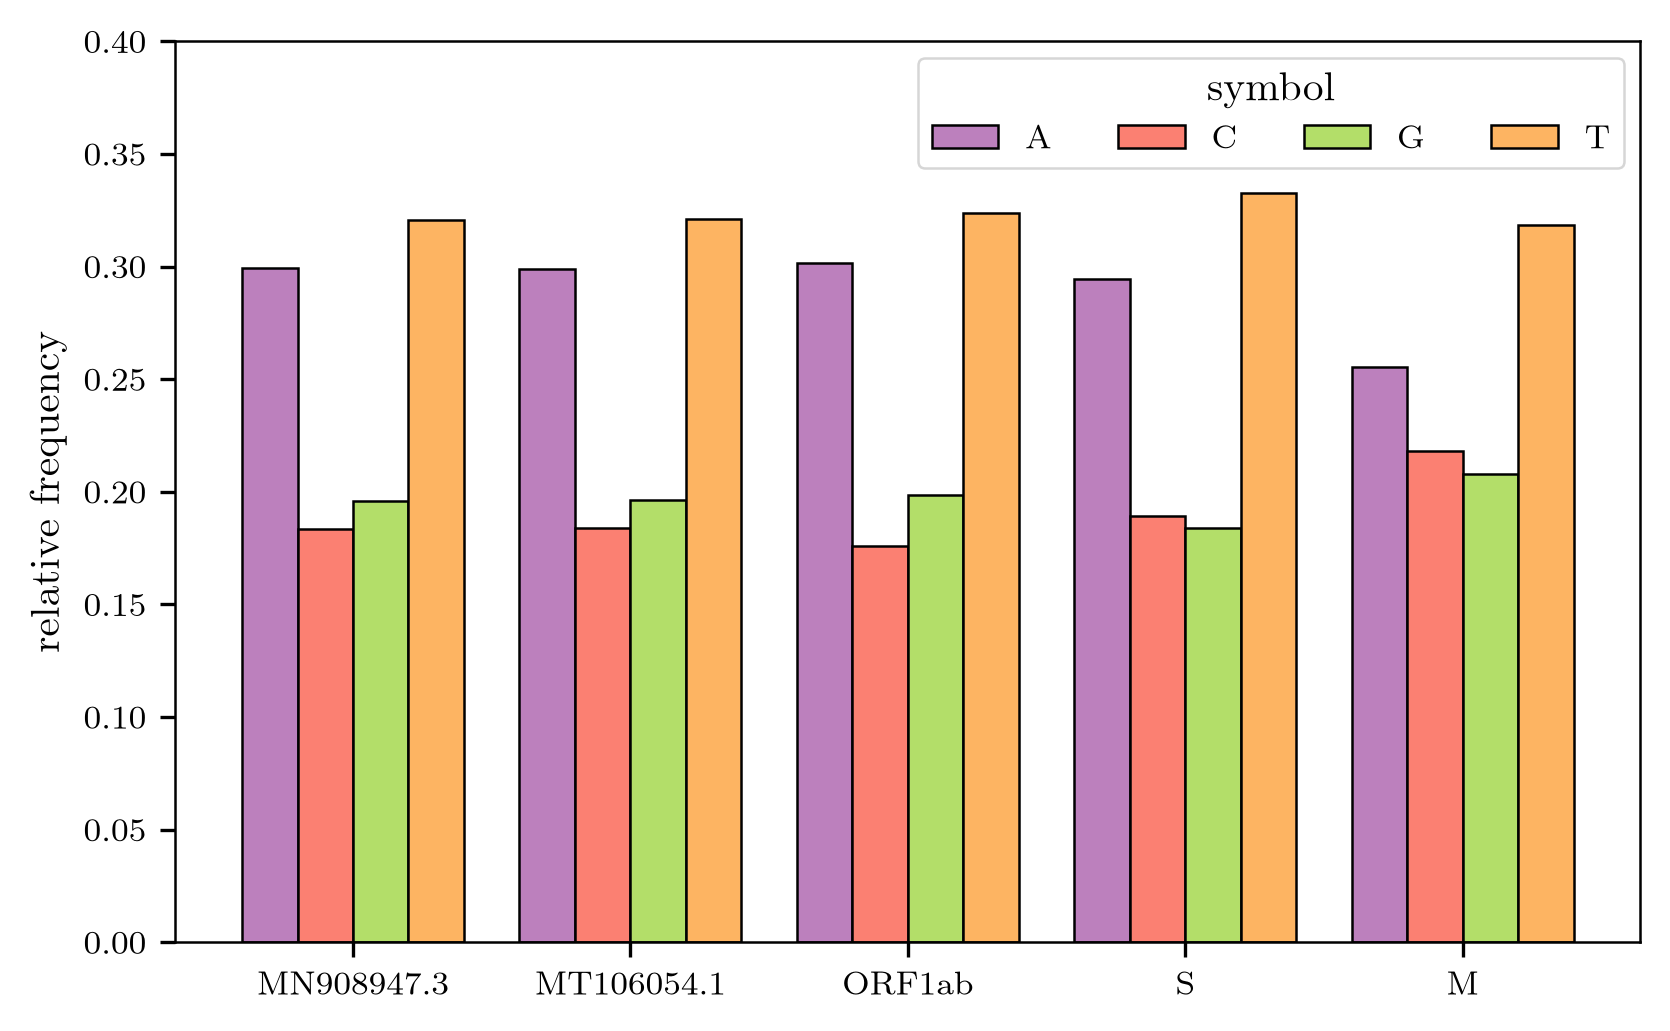
\includegraphics[width=0.6\textwidth]{fig_freq_dna}
    \caption{Relative nucleotide frequencies per DNA file.}
    \label{fig:freq}
\end{figure}

T is the most frequent base in every file. C is the least frequent in both genomes and in ORF1ab,
while in S and M the least frequent base is G. Gene M is the least skewed of the five DNA files. The
two genomes have practically identical composition (A 0.299, C 0.184, G 0.196, T 0.321 in both), a
first hint of how close they are before any alignment is computed. The amino-acid frequencies
(Figure~\ref{fig:freq_protein} in the appendix) are far from uniform: L is the most frequent and W
the least.

\section{Algorithm}\label{sec:algorithm}

\subsection{Longest common subsequence by dynamic programming}

For sequences $X = x_1 \dots x_n$ and $Y = y_1 \dots y_m$, the length of the longest common subsequence of the prefixes $x_1 \dots x_i$ and $y_1 \dots y_j$ satisfies
\begin{equation}
    L(i, j) = \begin{cases}
        0 & i = 0 \text{ or } j = 0, \\
        1 + L(i - 1, j - 1) & x_i = y_j, \\
        \max\big(L(i - 1, j),\, L(i, j - 1)\big) & x_i \ne y_j.
    \end{cases}
    \label{eq:lcs}
\end{equation}


The recurrence has overlapping subproblems. Each $L(i, j)$ is needed by up
to three other cells, so the naive recursion recomputes the same values exponentially many times. An
optimal solution for the pair $(i, j)$ contains an optimal solution for a smaller pair, which is what
makes the recurrence valid. A table filled row by row therefore costs $\Theta(nm)$
\citep{clrs}. The subsequence itself is recovered by tracing back through the table.

For the two genomes the table has $29\,903 \times 29\,882 \approx 8.9 \times 10^8$ cells, which is
3.6 GB at 4 bytes per cell, so the textbook algorithm cannot be run on a laptop or in Colab. The
length alone needs only two rows at a time, because a row depends only on the previous one. The
traceback, however, needs the whole table, so discarding the table also discards the alignment.

\subsection{Hirschberg: divide and conquer on top of the recurrence}

Hirschberg's algorithm removes the table without giving up the alignment \citep{hirschberg1975}. It
rests on three facts. First, the last row of the table, $L(\text{mid}, \cdot)$, can be computed with
two rows of memory. Second, for the split of $X$ at its midpoint,
$|LCS(X, Y)| = \max_k \big( |LCS(X[:\text{mid}], Y[:k])| + |LCS(X[\text{mid}:], Y[k:])| \big)$, and
the maximising $k$ is found by adding the forward last row of $X[:\text{mid}]$ against $Y$ to the
last row of the reversed $X[\text{mid}:]$ against the reversed $Y$. Third, once $k$ is fixed the two
halves are independent, so they are solved recursively and their results concatenated. Divide is the
split of $X$, while conquer is the recursion on the two sub-rectangles and combine is the concatenation.
Memory is $O(n + m)$ and time stays $O(nm)$, because the rectangles shrink geometrically
(Section~\ref{sec:complexity}).

Subproblems with at most $40\,000$ cells are solved with a full table and a traceback, which is the
base case of the recursion. On the two genomes the recursion produced 255 split points with a
maximum depth of 7 (Figure~\ref{fig:splits} in the appendix). A single-symbol $X$ is handled as its
own base case, so the split index is always at least 1 and every call makes progress.

\subsection{From subsequence to mutations}

Consecutive matched pairs $(i, j)$ and $(i', j')$ delimit an unmatched gap, $X[i+1:i']$ against
$Y[j+1:j']$. Because the LCS is optimal, the two sides of a gap share no symbol at all: a shared
symbol could be matched without disturbing any other pair, and the LCS would grow. A gap with equal length on both sides is therefore a run of substitutions, a gap with one
empty side is an insertion or a deletion, and anything else is a complex change.



Each substitution inside a coding region is translated in both genomes with the standard genetic
code and classified as synonymous or non-synonymous. The reading frames are not assumed. Gene S and
gene M translate exactly to their protein records, and ORF1ab is translated in two frames because of
the ribosomal frameshift at position 13\,468: the ORF1a frame from 266 and the ORF1b frame from
13\,468. Ten protein records are found whole in the first frame and four in the second, which
validates both the frames and the codon table. Once backtracking (below) locates every protein, the
classification is repeated over all coding regions.

\subsection{Supporting techniques}

Naive search tries every alignment and compares symbol by symbol, which is $O(nm)$ in the worst
case. KMP preprocesses the pattern into its failure table, so that after a mismatch the text pointer
never moves backwards \citep{kmp1977}. The Z-function computes, for \texttt{pattern + \# + text}, the
length of the longest prefix match at every position, and a value equal to $m$ is an occurrence. Both
are $O(n + m)$. The improved methods avoid the repeated work of naive search because after a mismatch
they reuse what is already known about the pattern instead of restarting the comparison.

We consider every open reading frame of at least 100 codons in the three forward frames, each
running from an ATG to the next in-frame stop. Picking the largest set of these that do not
overlap is the activity selection problem. The greedy rule sorts candidates by end position and
keeps each one that does not overlap the last one kept. This is optimal (CLRS ch.~16): the
earliest-ending interval can always replace the first interval of an optimal solution without
creating an overlap. The limitation appears in the results: the objective is the
count of intervals, not the coverage of the genome.

The genetic code has up to six codons per amino acid, so a protein of length $L$
has up to $6^L$ encodings. The search builds an encoding codon by codon. The state of a node is the
set of genome positions still consistent with the codons chosen so far, and a choice that leaves that
set empty is pruned together with its whole subtree. Only the first $k = 6$ amino acids are searched
this way. Every surviving position is then verified by translating the genome forward for the whole
protein.

The candidates are $k$-mers built symbol by symbol, so the search space is a tree of
prefixes. A node carries the genome positions whose window still agrees with the prefix within $d$
mismatches, and the number of those positions is a valid upper bound on the count of any completion
of the prefix, because a window within $d$ mismatches of the full $k$-mer is within $d$ mismatches of
its prefix. Nodes are expanded best first from a max-heap ordered by that bound, the incumbent comes
from a greedy descent, and a node is pruned when its bound cannot beat the incumbent. A hash table is
not used because with $d = 0$ a single pass over the genome solves the problem in $O(nk)$, which is
why the mismatch version is the one that justifies branch and bound.

Centre expansion tries the $2n - 1$ possible centres and is $O(n^2)$ in the worst case. Manacher's
algorithm interleaves a separator so that every palindrome has odd length, then reuses the radius of
the mirror centre inside the rightmost known palindrome \citep{manacher1975}. Each symbol extends the
right boundary at most once, so the algorithm is $O(n)$.

\section{Implementation}\label{sec:implementation}

\ph{Overview paragraph. Main idea: a single notebook, \texttt{dna\_analysis.ipynb}, runs from top to bottom with no manual edits, in Jupyter or Colab, and needs only numpy and matplotlib. Every string algorithm is written from scratch: no \texttt{str.find}, no library search or alignment; numpy is used only to vectorise a dynamic programming row and for plotting. The notebook writes every figure and every table of this report into \texttt{figures/} and \texttt{tables/}, so no number was typed by hand.}

The main components are: \texttt{read\_fasta} and \texttt{characterize} (parsing, Part 1 statistics, the unexpected-symbol check); \texttt{naive\_search}, \texttt{kmp\_search} with \texttt{build\_lps}, \texttt{z\_search} with \texttt{z\_function}, and \texttt{search\_all}, which runs the three and asserts that they agree; \texttt{lcs\_table} (full table with traceback, the oracle), \texttt{lcs\_rows\_py} (two rows, pure Python), \texttt{lcs\_last\_row} (two rows, numpy) and \texttt{hirschberg}, which returns the matched index pairs; \texttt{alignment\_events}, \texttt{classify\_substitutions} and \texttt{translate} with the standard codon table; \texttt{find\_orfs}, \texttt{greedy\_select}, \texttt{exhaustive\_select}; \texttt{locate\_backtracking}, \texttt{locate\_bruteforce} and \texttt{matched\_prefix} on top of a codon index (a dictionary from every 3-mer to its positions); \texttt{motif\_bnb} and \texttt{motif\_exhaustive} sharing \texttt{motif\_children}; \texttt{longest\_palindrome\_center} and \texttt{manacher}; and \texttt{bench} (minimum of repeated runs with \texttt{perf\_counter}) with \texttt{loglog\_slope}.

\ph{The numpy row trick. Main idea: a row of the LCS table is a running maximum. When $x_i = y_j$ the diagonal value plus one dominates both neighbours; otherwise the cell is the maximum of its two neighbours. So with $c_j = L(i-1, j-1) + 1$ if $x_i = y_j$ and $c_j = L(i-1, j)$ otherwise, the row is $L(i, j) = \max(c_j, L(i, j-1))$, a cumulative maximum that numpy computes with \texttt{maximum.accumulate} in one vectorised call per row. This is what makes Hirschberg run on two full genomes in a few seconds of Python.}

\ph{Correctness checks (all are assertions in the notebook and all pass). Notes: the three search methods return identical positions on every search and the gene positions equal the header coordinates minus one; the LCS implementations (full table, two rows in Python, two rows in numpy, Hirschberg) agree with each other and with an independent bit-parallel oracle on the textbook example, on 200 random strings with the recursion forced down to tiny base cases, and on four genome windows containing substitutions, shifts and unequal lengths; on the full genomes the Hirschberg pairs form a valid common subsequence whose length equals the oracle's; gene S and gene M translate exactly to their protein records; greedy equals the exhaustive optimum on 14 candidates spread over the genome; backtracking and brute force find the same positions for every protein; branch and bound equals exhaustive search at $k = 8$, and with $d = 0$ equals a hash count; Manacher equals centre expansion on the three genes.}

\section{Complexity analysis}\label{sec:complexity}

\ph{LCS paragraph. Main idea: filling the table is $\Theta(nm)$ time and $\Theta(nm)$ space; the length alone is $\Theta(nm)$ time and $\Theta(m)$ space. For the genomes: $8.9 \times 10^8$ cells, 3.57 GB as a table, 239 KB as two rows.}

\ph{Hirschberg paragraph. Main idea: at the top level the two last-row computations cost $nm$ cell updates; at the next level the two sub-rectangles have total area at most $nm / 2$ because they split both $X$ and $Y$; the areas form a geometric series, so the total is at most $2nm$ cell updates, that is, $O(nm)$ time with $O(n + m)$ memory. Depth is $O(\log n)$. Note the constant: about twice the work of the length-only version, which is what the measurements show (Table~\ref{tab:complexity}).}

\ph{Pattern search paragraph. Naive: $O(nm)$ worst case, reached by the adversarial text $A^n$ with pattern $A^{m-1}C$; on real DNA a mismatch occurs after about $1.3$ comparisons on average so it behaves linearly. KMP: $O(m)$ preprocessing plus $O(n)$ scan, because the text pointer only advances and the pattern pointer decreases at most as often as it increases. Z: $O(n + m)$ by the same amortised argument on the right boundary.}

\ph{Greedy, backtracking, branch and bound paragraph. Greedy ORF selection: $O(n)$ to scan the three frames, $O(c \log c)$ to sort $c$ candidates, versus $O(2^c)$ for the exhaustive subset search (doubling per candidate is visible in Figure~\ref{fig:search_space}). Backtracking: worst case is the number of encodings, $\prod_{t \le k} \deg(a_t) \le 6^k$, but each node costs only the size of its candidate set, and pruning keeps the explored nodes near-constant in $k$ once the prefix is specific enough. Branch and bound: worst case $O(4^k \cdot n)$ like exhaustive search; the measured benefit is on nodes, not on time, because the bound $|\text{alive}|$ is loose at shallow depth, where most positions are still alive and most of the filtering work happens.}

\ph{Manacher paragraph. Centre expansion $O(n^2)$ worst case (slope 2.00 on $A^n$), Manacher $O(n)$ (slope 1.05 on the same input). On real DNA both are effectively linear because palindromes are short, so Manacher's advantage only shows on adversarial input.}

\section{Results}\label{sec:results}

\subsection{Genome comparison}

\begin{table}[H]
    \centering
    \small
    \begin{tabular}{lr}
\hline
MN908947.3 (Wuhan) length & 29903 \\
MT106054.1 (Texas) length & 29882 \\
$|LCS|$ & 29875 \\
similarity $|LCS| / \max(n, m)$ & 0.99906 \\
substituted positions & 6 \\
\quad synonymous & 3 \\
\quad non-synonymous & 3 \\
\quad outside coding regions & 0 \\
insertions / deletions / complex & 1 / 2 / 0 \\
Hirschberg time (alignment) & 3.9 s \\
full DP table memory (not run) & 3.6 GB \\
\hline
\end{tabular}
    \caption{Wuhan 2019 versus Texas 2020 by longest common subsequence.}
    \label{tab:genome}
\end{table}

\ph{What the number means. Main idea: $|LCS| = 29\,875$ against lengths 29\,903 and 29\,882 gives a similarity of 0.99906; the LCS counts symbols that can be kept in order in both genomes, so $n - |LCS| = 28$ symbols of Wuhan and $m - |LCS| = 7$ of Texas have no partner. Limitation to state: the LCS ignores locality, a scattered set of matches and a contiguous block score the same, which is why the gap analysis is needed to say where the differences are.}

\begin{table}[H]
    \centering
    \small
    \begin{tabular}{rrcclcl}
\hline
Wuhan pos & Texas pos & base & region & codon & amino acid & effect \\
\hline
8782 & 8782 & C$\to$T & QHD43415\_4 & AGC$\to$AGT & S$\to$S & synonymous \\
18603 & 18603 & T$\to$C & QHD43415\_13 & CAT$\to$CAC & H$\to$H & synonymous \\
18975 & 18975 & T$\to$A & QHD43415\_13 & GTT$\to$GTA & V$\to$V & synonymous \\
19175 & 19175 & A$\to$C & QHD43415\_13 & GAT$\to$GCT & D$\to$A & non-synonymous \\
27925 & 27925 & C$\to$T & QHD43422 & ACA$\to$ATA & T$\to$I & non-synonymous \\
28144 & 28144 & T$\to$C & QHD43422 & TTA$\to$TCA & L$\to$S & non-synonymous \\
\hline
\end{tabular}
    \caption{Substitutions between the two genomes (1-based positions) and their effect on the encoded amino acid.}
    \label{tab:mutations}
\end{table}

\begin{figure}[H]
    \centering
    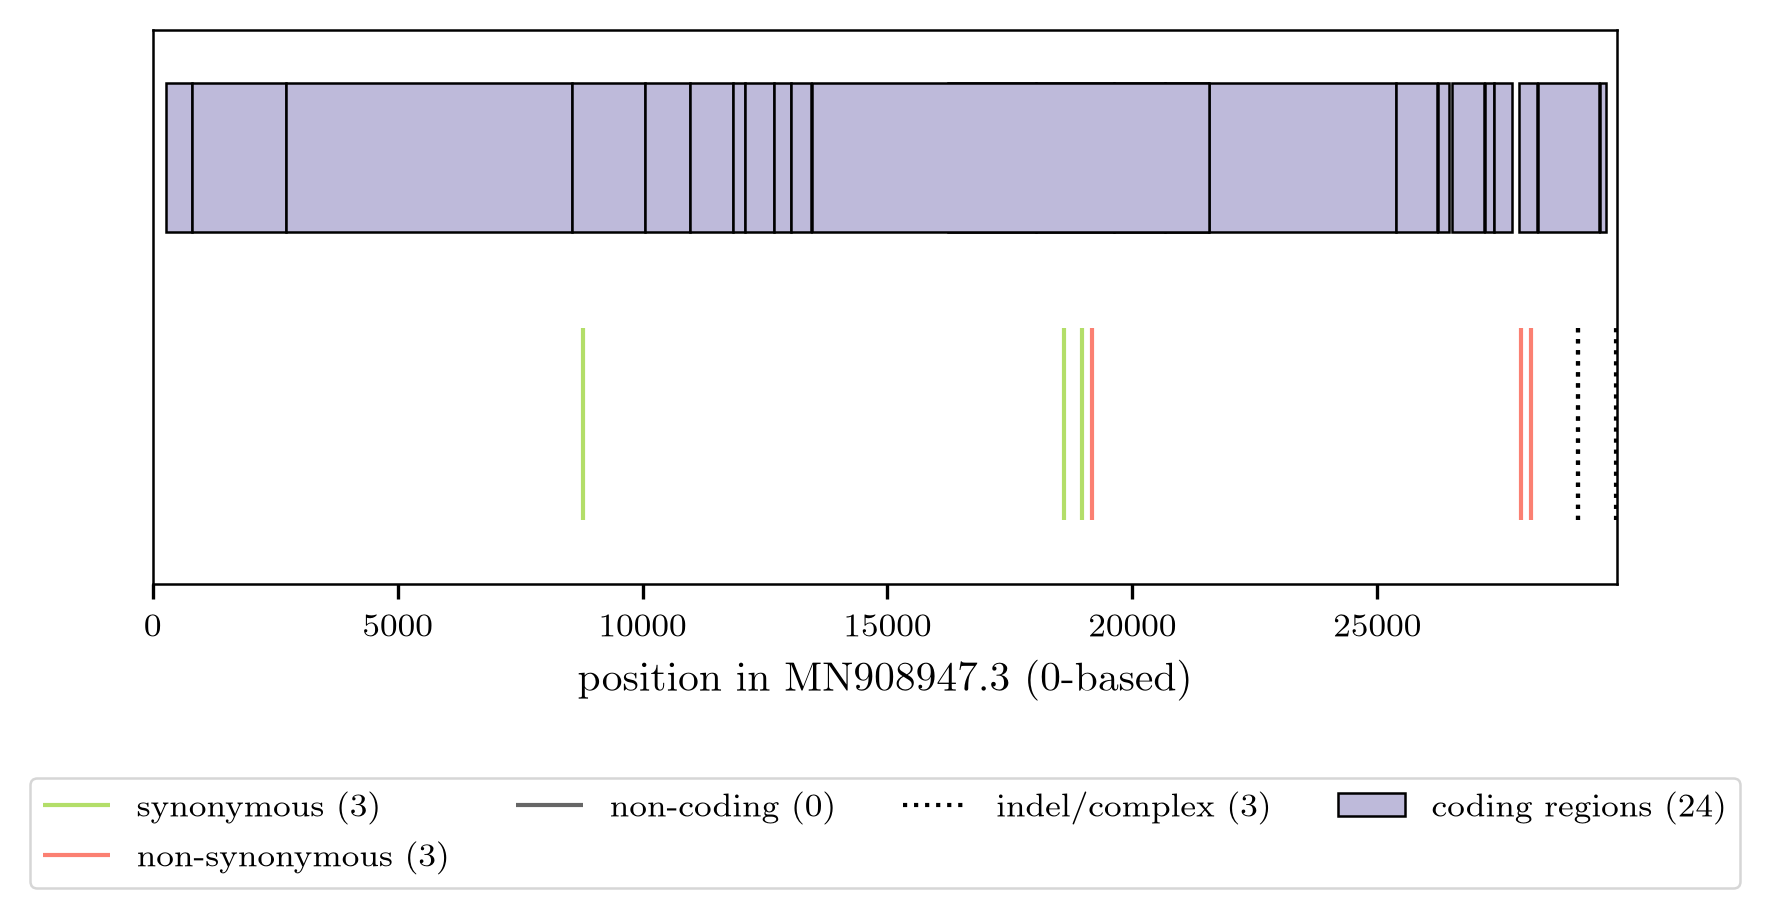
\includegraphics[width=0.72\textwidth]{fig_mutation_map}
    \caption{Position of every difference along the Wuhan genome, with the coding regions located by backtracking.}
    \label{fig:mutations}
\end{figure}

\ph{Reading Table~\ref{tab:mutations} and Figure~\ref{fig:mutations}. Main idea: six substitutions, three synonymous and three non-synonymous; the non-synonymous ones are D$\to$A in QHD43415\_13 and two in QHD43422 (T$\to$I, L$\to$S). The three indels are all after position 29\,000: a 21-nucleotide run of A missing from the Texas record, which is the poly-A tail (how far the sequencing read, not a mutation), and an insertion plus a deletion three positions apart near 29\,091 that is really one more substitution, C$\to$T at 29\,095: the LCS has no substitution operation, and when the changed base equals its neighbour (Wuhan \texttt{GCTTTCGG}, Texas \texttt{GCTTTTGG}) an indel pair and a substitution give the same LCS length, so the traceback may return either. This is the main limitation of using the LCS as a diff. Note that two substitutions fell outside the three gene files and could only be classified after backtracking located QHD43422.}

\subsection{Search, greedy, backtracking, branch and bound, palindromes}

\ph{One paragraph per technique, numbers from the appendix tables. Search: all three genes found at exactly the header coordinates (ORF1ab at 266, S at 21\,563, M at 26\,523, 1-based), and in the Texas genome S and M are found intact while ORF1ab is not, consistent with the substitutions in Table~\ref{tab:mutations}. Greedy: 187 candidate ORFs, 8 selected, S and M recovered exactly, ORF1a and ORF1b as the two large pieces; lowering the threshold to 30 codons makes greedy pick 53 small ORFs covering 30\% of the genome and none of the known genes, because the objective is the count (Table~\ref{tab:orfs}, Figure~\ref{fig:orf}). Backtracking: 23 of 24 proteins located over their full length with a few dozen nodes each; the exception, QHD43415\_11, matches exactly 9 amino acids from position 13\,441, that is, up to nucleotide 13\,468, the ribosomal frameshift, so the algorithm found the biology rather than failing (Table~\ref{tab:proteins}). Branch and bound: for $k = 8$, $d = 1$ the motif TGTTGTTA occurs 75 times, the same optimum as exhaustive search with 6\,383 instead of 85\,695 nodes (Table~\ref{tab:motif}). Palindromes: longest palindrome of 11, 15 and 20 nucleotides in M, S and ORF1ab (Table~\ref{tab:palindromes}).}

\subsection{Performance}

\begin{figure}[H]
    \centering
    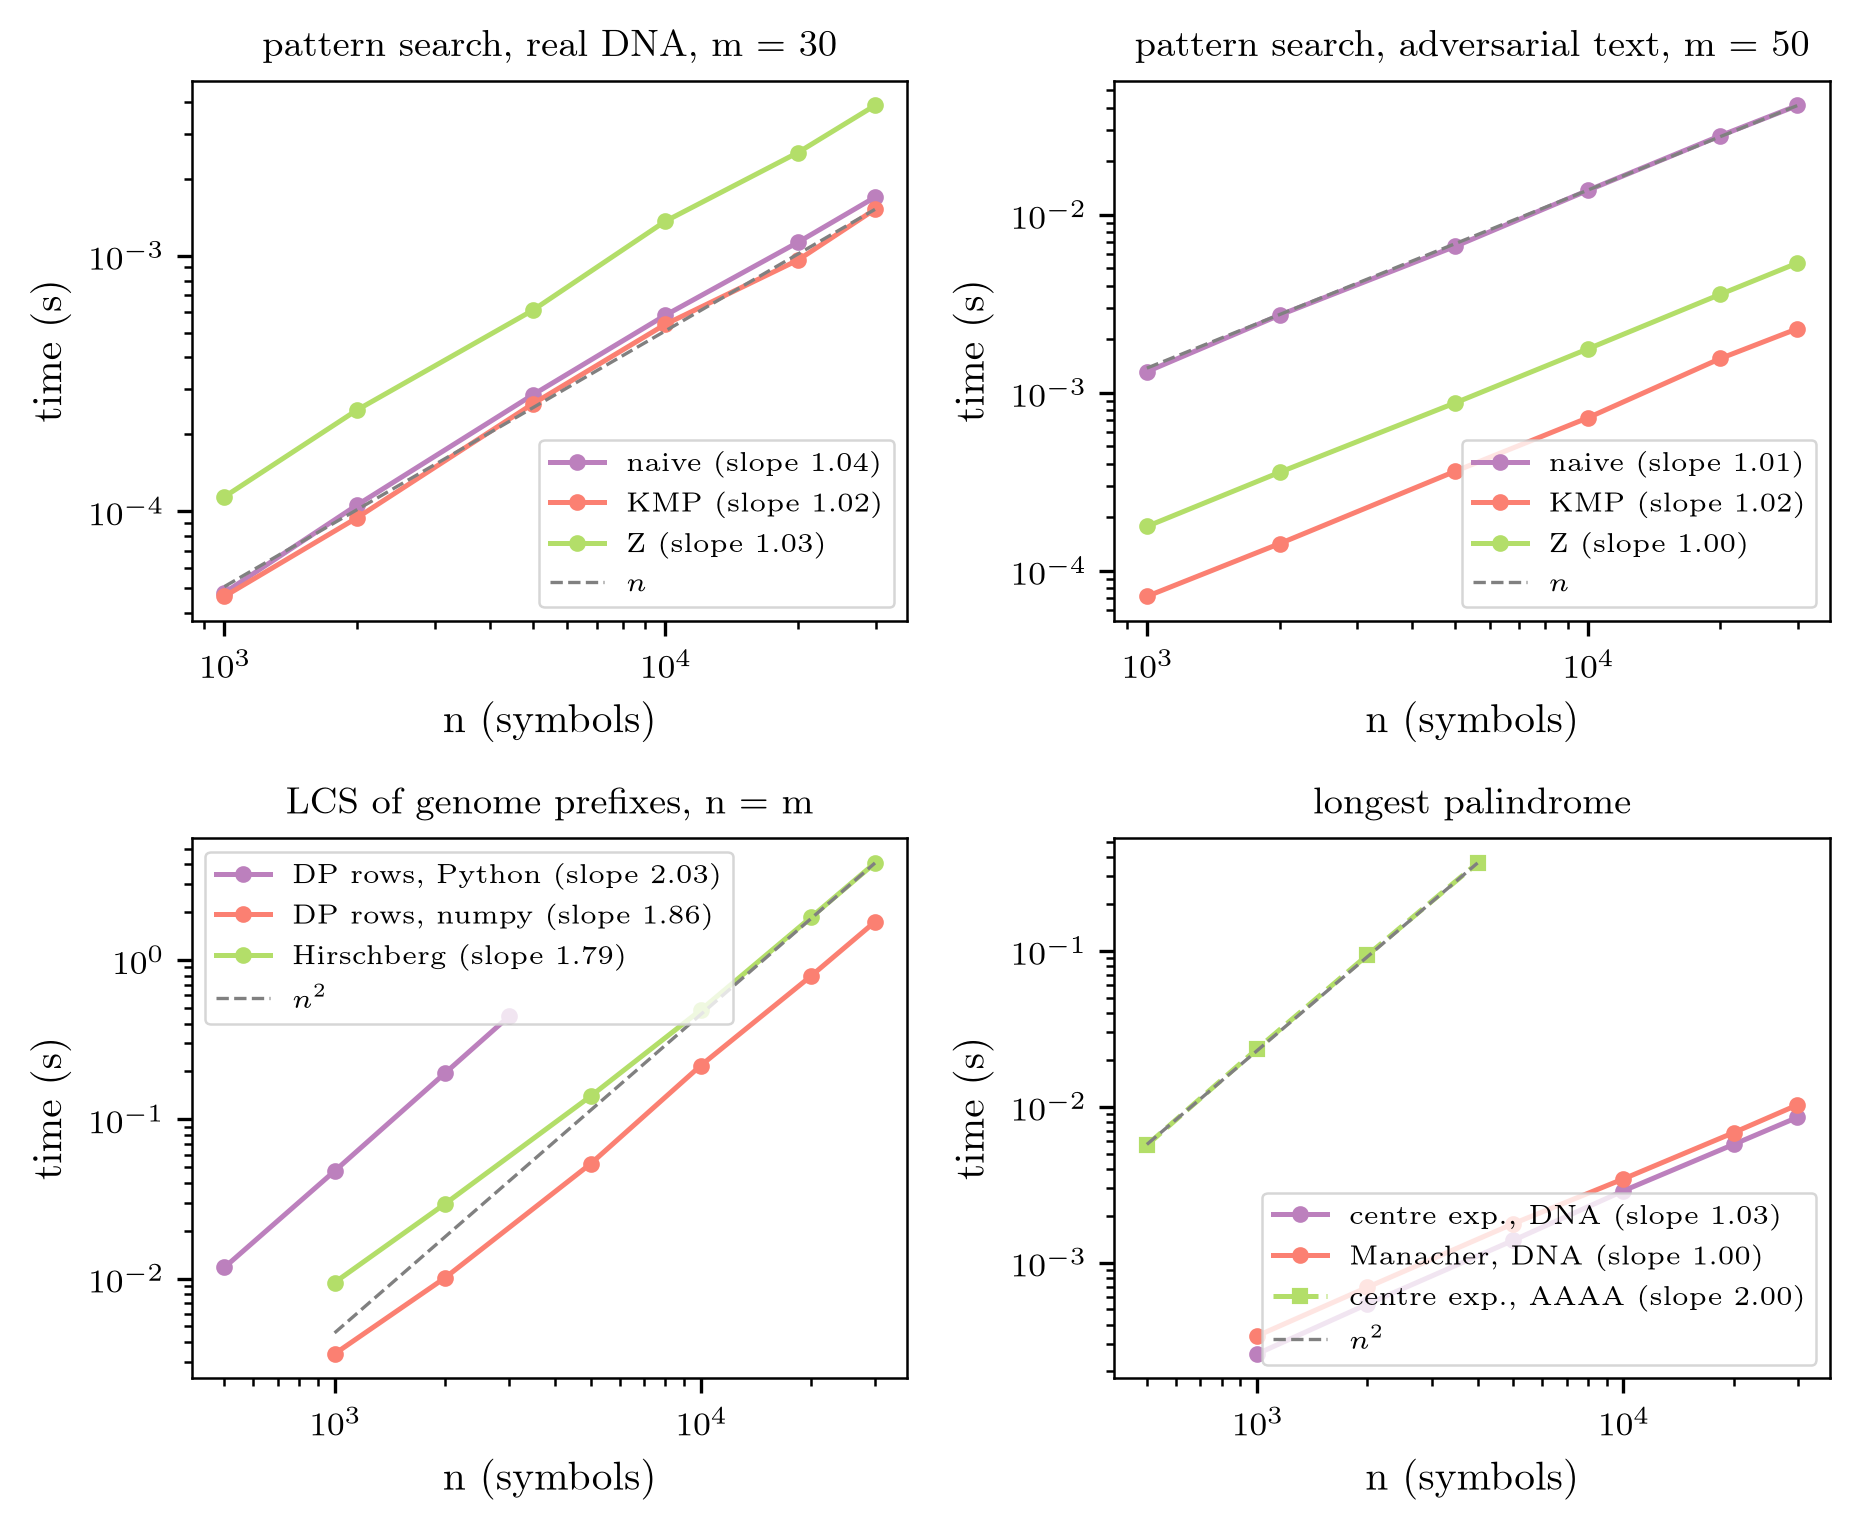
\includegraphics[width=0.8\textwidth]{fig_time_scaling}
    \caption{Running time against input size (log-log). Dashed lines are the theoretical growth anchored at the largest measurement; slopes in the legends are least-squares fits.}
    \label{fig:time}
\end{figure}

\ph{Explain Figure~\ref{fig:time} panel by panel. Search on real DNA: all three linear (slopes close to 1, Table~\ref{tab:complexity}); naive is not slower because a mismatch ends most alignments after one or two comparisons; Z is two to three times KMP because it builds and stores an array of $n + m + 1$ values while KMP keeps one pointer. Adversarial text: naive is still slope 1 in $n$ but 20 times slower than KMP, the factor $m = 50$ of the $O(nm)$ bound; KMP and Z unchanged. LCS: pure Python rows and numpy rows both have slope close to 2, quadratic as $O(nm)$ with $n = m$; Hirschberg has the same slope and costs about twice the numpy rows, the $2nm$ bound; the pure Python version reaches only $n = 3\,000$ in the time numpy needs for the full genomes. Palindromes: centre expansion linear on DNA (1.02) but quadratic on $A^n$ (2.00); Manacher linear on both.}

\begin{figure}[H]
    \centering
    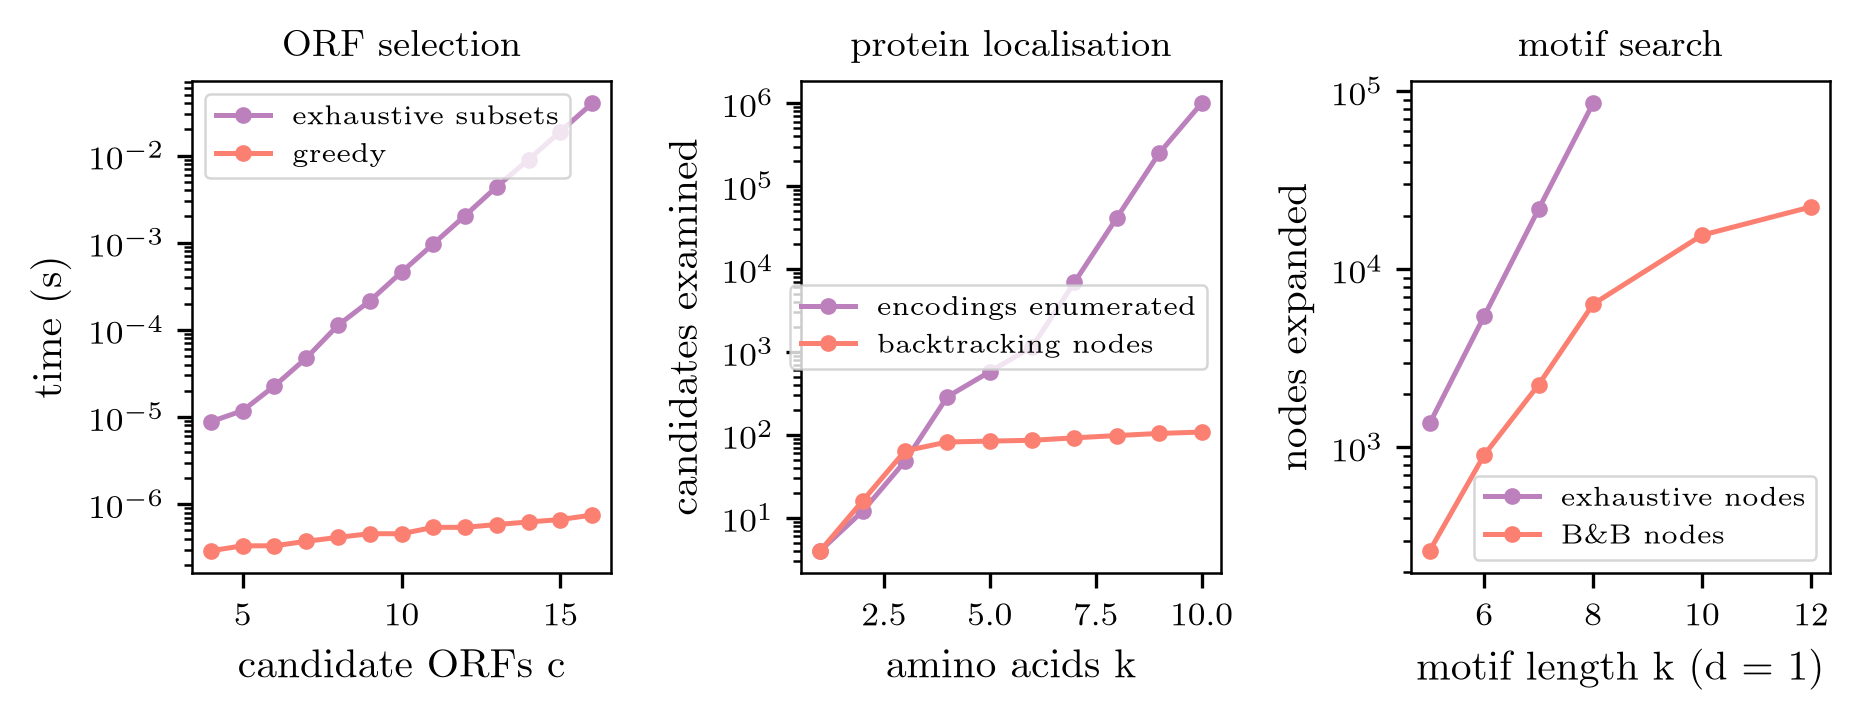
\includegraphics[width=0.85\textwidth]{fig_search_space}
    \caption{Search-space techniques against their baselines: exhaustive subsets versus greedy, encodings enumerated versus backtracking nodes, exhaustive versus branch-and-bound nodes.}
    \label{fig:search_space}
\end{figure}

\ph{Explain Figure~\ref{fig:search_space}. Exhaustive subset search doubles with every candidate while greedy is flat; enumerating encodings grows by the codon degeneracy at each amino acid (up to $10^6$ at $k = 10$) while backtracking stays near 100 nodes because after three amino acids the prefix pins down a single genome position; branch and bound expands about 7\% of the exhaustive nodes at $k = 8$ and keeps growing slowly to $k = 12$, where exhaustive search is no longer feasible.}

\section{Conclusions}\label{sec:conclusions}

\ph{Bullet-style conclusions to expand, one per technique, then the comparison.
(1) Dynamic programming gives the exact answer but its table is the bottleneck; divide and conquer did not change the time bound, it changed what fits in memory, and that is what made the full-genome comparison possible.
(2) The linear-time string algorithms only pay off when the pattern is repetitive; on real DNA brute force is already linear in practice, so the theoretical worst case is what justifies KMP, not the average run.
(3) Greedy is provably optimal for the objective it is given, and the ORF experiment shows that the objective is the whole story: maximum count and maximum coverage are different problems.
(4) Backtracking turns an exponential enumeration into a few dozen nodes because the genome is a very strong constraint; its one apparent failure was the frameshift, a fact about the data.
(5) Branch and bound is only as good as its bound: the same optimum, far fewer nodes, but no time saved because the bound is loose where the work is.
(6) Manacher is the only technique whose advantage was invisible on the real data and visible only under an adversarial input.
Comparison across techniques: which scaled best (linear string algorithms and greedy), which needed the most resources (LCS, quadratic, and exhaustive baselines), whether datasets changed the behaviour (yes: real DNA versus adversarial input flips the naive-vs-KMP and centre-vs-Manacher comparisons; the threshold flips the greedy result).}

\ph{Closing paragraph: what was learned about relating experiment to theory: log-log slopes reproduce the exponents, constants matter (numpy versus Python, $2nm$ versus $nm$), and the baseline must be run to know whether the sophisticated algorithm was needed.}


\addcontentsline{toc}{section}{References}
\bibliographystyle{apalike}
\bibliography{references}

\pagebreak
\begin{appendices}
\addcontentsline{toc}{section}{Appendix}

\section{Additional tables}

\begin{table}[H]
    \centering
    \scriptsize
    \renewcommand{\arraystretch}{1.25}
    \setlength{\tabcolsep}{3pt}
    \begin{tabular}{>{\raggedright\arraybackslash}p{2.6cm}>{\raggedright\arraybackslash}p{2.5cm}>{\raggedright\arraybackslash}p{3.9cm}>{\raggedright\arraybackslash}p{1.3cm}>{\raggedright\arraybackslash}p{1.1cm}>{\raggedright\arraybackslash}p{3.7cm}}
\hline
algorithm & technique & complexity & slope real & slope adv. & largest run (real / adv.) \\
\hline
naive search & brute force & $O(nm)$ & 1.03 & 1.03 & 1.6 ms / 39.4 ms, $n = 29903$ \\
KMP & string & $O(n + m)$ & 1.00 & 1.00 & 1.4 ms / 2.0 ms, $n = 29903$ \\
Z-function & string & $O(n + m)$ & 1.01 & 1.00 & 3.4 ms / 4.8 ms, $n = 29903$ \\
LCS rows, Python & DP & $O(nm)$ time, $O(m)$ space & 2.08 & -- & 438.5 ms, $n = 3000$ \\
LCS rows, numpy & DP & $O(nm)$ time, $O(m)$ space & 1.86 & -- & 1.63 s, $n = 29903$ \\
Hirschberg & D\&C + DP & $O(nm)$ time, $O(n + m)$ space & 1.78 & -- & 3.80 s, $n = 29903$ \\
ORF selection & greedy & $O(n + c \log c)$ vs $O(2^c)$ & 1.04 (scan) & -- & exhaustive 38.6 ms, $c = 16$ \\
protein localisation & backtracking & $O(6^k)$ worst, pruned & -- & -- & 108 vs 995328 nodes, $k = 10$ \\
motif search & branch and bound & $O(4^k n)$ worst, pruned & -- & -- & 6383 vs 85695 nodes, $k = 8$ \\
centre expansion & brute force & $O(n^2)$ & 1.05 & 2.00 & 8.3 ms / 364.8 ms \\
Manacher & string & $O(n)$ & 1.04 & 1.04 & 10.6 ms / 1.6 ms \\
\hline
\end{tabular}
    \caption{Theoretical complexity against the measured log-log slope of running time versus input size. Timings from one run of the notebook on a laptop.}
    \label{tab:complexity}
\end{table}

\begin{table}[H]
    \centering
    \scriptsize
    \begin{tabular}{lrrrrrrr}
\hline
protein & length & start & end & frame & matched & nodes & pruned \\
\hline
QHD43415\_1 & 180 & 265 & 805 & 1 & 180/180 & 41 & 32 \\
QHD43415\_2 & 638 & 805 & 2719 & 1 & 638/638 & 86 & 65 \\
QHD43415\_3 & 1945 & 2719 & 8554 & 1 & 1945/1945 & 76 & 56 \\
QHD43415\_4 & 500 & 8554 & 10054 & 1 & 500/500 & 41 & 27 \\
QHD43415\_5 & 306 & 10054 & 10972 & 1 & 306/306 & 97 & 66 \\
QHD43415\_6 & 290 & 10972 & 11842 & 1 & 290/290 & 140 & 103 \\
QHD43415\_7 & 83 & 11842 & 12091 & 1 & 83/83 & 56 & 31 \\
QHD43415\_8 & 198 & 12091 & 12685 & 1 & 198/198 & 86 & 64 \\
QHD43415\_9 & 113 & 12685 & 13024 & 1 & 113/113 & 42 & 30 \\
QHD43415\_10 & 139 & 13024 & 13441 & 1 & 139/139 & 68 & 45 \\
QHD43415\_11 & 932 & 13441 & 16237 & 1 & 9/932 & 90 & 58 \\
QHD43415\_12 & 601 & 16236 & 18039 & 0 & 601/601 & 102 & 76 \\
QHD43415\_13 & 527 & 18039 & 19620 & 0 & 527/527 & 42 & 26 \\
QHD43415\_14 & 346 & 19620 & 20658 & 0 & 346/346 & 142 & 87 \\
QHD43415\_15 & 298 & 20658 & 21552 & 0 & 298/298 & 143 & 93 \\
QHD43416 & 1273 & 21562 & 25381 & 1 & 1273/1273 & 25 & 17 \\
QHD43417 & 275 & 25392 & 26217 & 0 & 275/275 & 26 & 18 \\
QHD43418 & 75 & 26244 & 26469 & 0 & 75/75 & 29 & 21 \\
QHD43419 & 222 & 26522 & 27188 & 2 & 222/222 & 37 & 26 \\
QHD43420 & 61 & 27201 & 27384 & 0 & 61/61 & 23 & 15 \\
QHD43421 & 121 & 27393 & 27756 & 0 & 121/121 & 23 & 15 \\
QHD43422 & 121 & 27893 & 28256 & 2 & 121/121 & 19 & 12 \\
QHD43423 & 419 & 28273 & 29530 & 1 & 419/419 & 31 & 19 \\
QHI42199 & 38 & 29557 & 29671 & 1 & 38/38 & 22 & 13 \\
\hline
\end{tabular}
    \caption{Proteins located by backtracking with $k = 6$ amino acids (0-based genome positions). Matched is the number of leading amino acids reproduced by translating the genome from the located start.}
    \label{tab:proteins}
\end{table}

\begin{table}[H]
    \centering
    \small
    \begin{tabular}{rrrrl}
\hline
start & end & frame & codons & known gene overlap \\
\hline
265 & 13483 & 1 & 4405 & ORF1ab (62\%) \\
13767 & 21555 & 0 & 2595 & ORF1ab (37\%) \\
21562 & 25384 & 1 & 1273 & S (100\%) \\
25392 & 26220 & 0 & 275 & - \\
26522 & 27191 & 2 & 222 & M (100\%) \\
27393 & 27759 & 0 & 121 & - \\
27893 & 28259 & 2 & 121 & - \\
28273 & 29533 & 1 & 419 & - \\
\hline
\end{tabular}
    \caption{ORFs selected by greedy activity selection among candidates with at least 100 codons (0-based positions).}
    \label{tab:orfs}
\end{table}

\begin{table}[H]
    \centering
    \small
    \begin{tabular}{rrlrrr}
\hline
$k$ & $d$ & best motif & count & exhaustive nodes & B\&B nodes \\
\hline
5 & 1 & TTTTT & 1241 & 1365 & 263 \\
6 & 1 & TTTTTT & 418 & 5461 & 907 \\
7 & 1 & TGTTGTT & 193 & 21836 & 2252 \\
8 & 1 & TGTTGTTA & 75 & 85695 & 6383 \\
10 & 1 & AAAAGAAAAA & 33 & -- & 15575 \\
12 & 1 & AAAAAAAAAAAA & 24 & -- & 22445 \\
\hline
\end{tabular}
    \caption{Most frequent $k$-mer with up to one mismatch in the Wuhan genome.}
    \label{tab:motif}
\end{table}

\begin{table}[H]
    \centering
    \small
    \begin{tabular}{lrlrrr}
\hline
gene & length & longest palindrome & start & end & length \\
\hline
M & 669 & \texttt{CTAAAGAAATC} & 493 & 504 & 11 \\
S & 3822 & \texttt{GAATTTGTGTTTAAG} & 570 & 585 & 15 \\
orf1ab & 21290 & \texttt{CTCAATGACTTCAGTAACTC} & 9711 & 9731 & 20 \\
\hline
\end{tabular}
    \caption{Longest palindrome per gene (0-based positions inside the gene).}
    \label{tab:palindromes}
\end{table}

\section{Additional figures}

\begin{figure}[H]
    \centering
    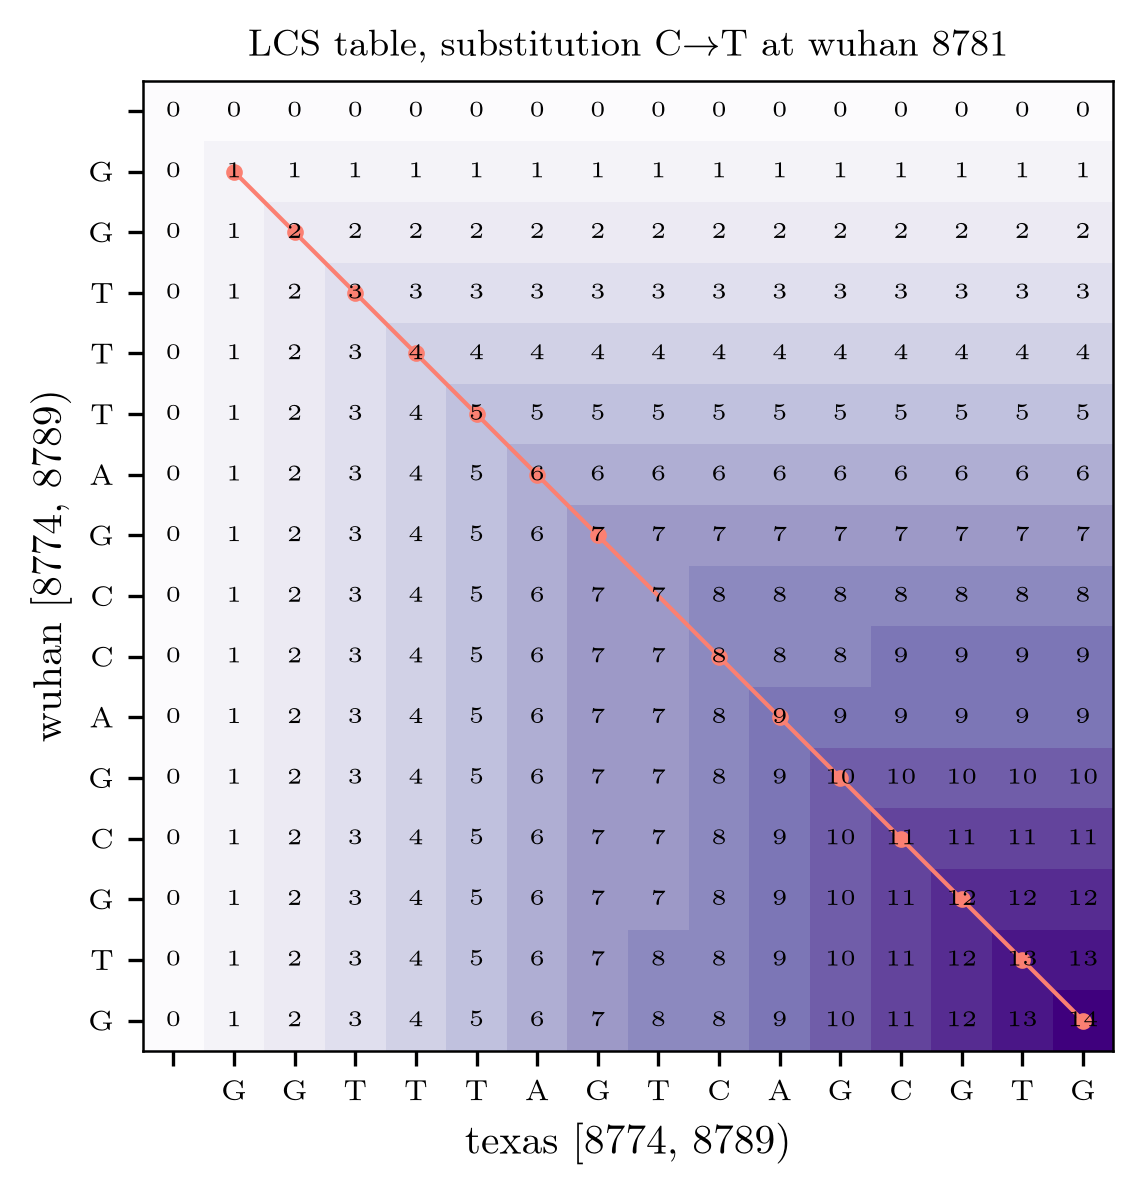
\includegraphics[width=0.48\textwidth]{fig_lcs_matrix}
    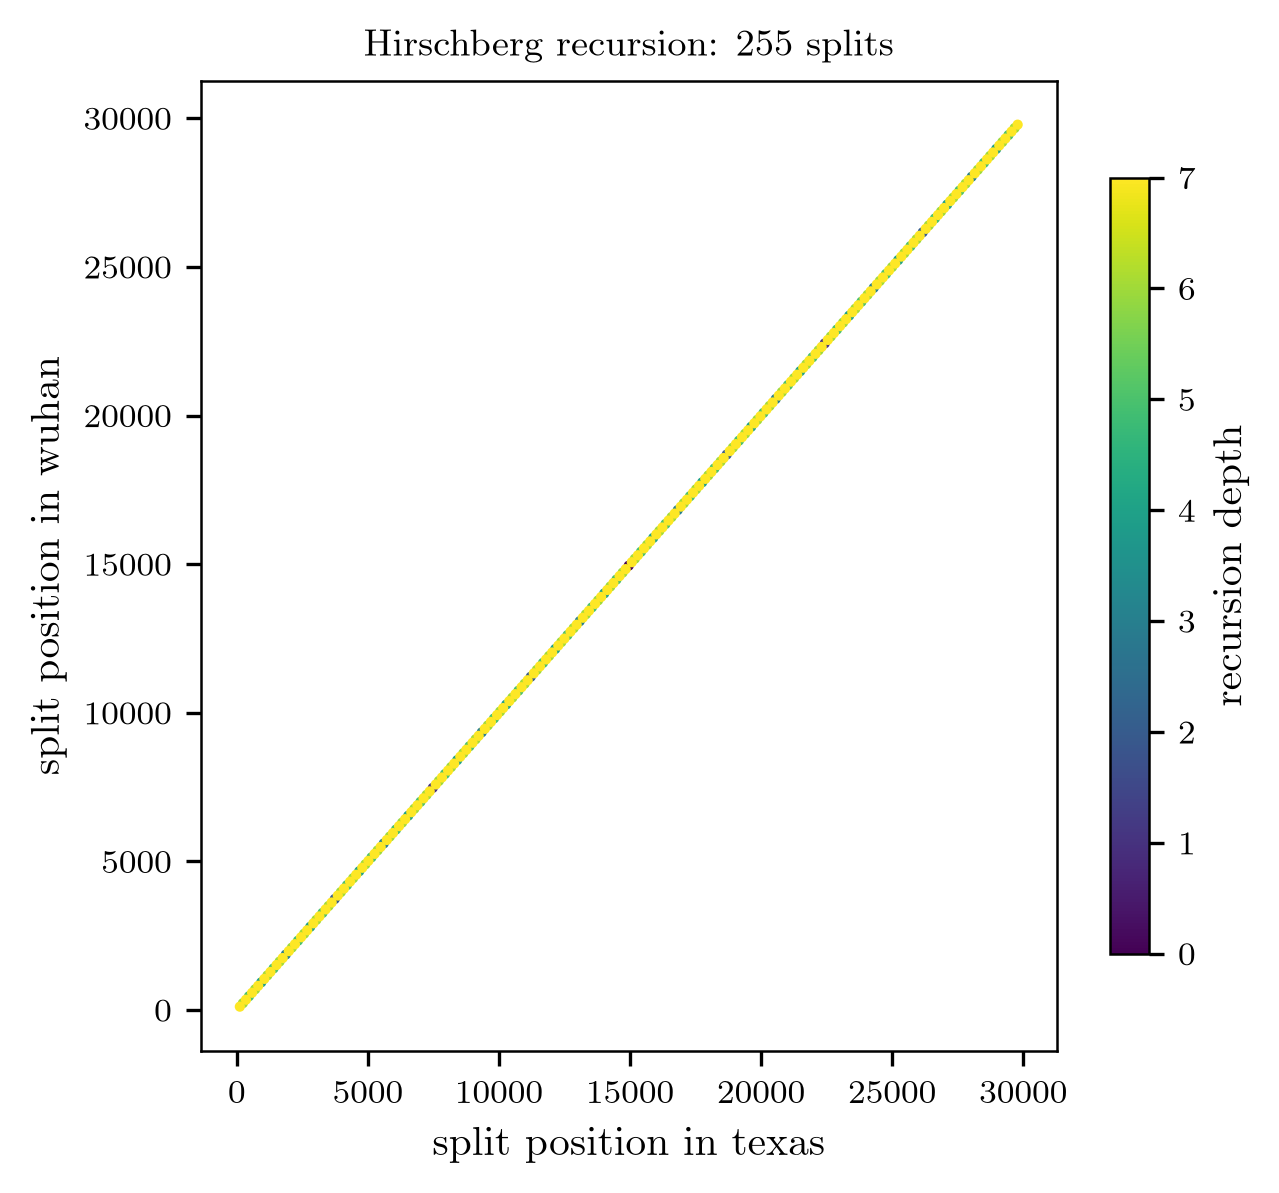
\includegraphics[width=0.48\textwidth]{fig_hirschberg_splits}
    \caption{Left: LCS table and traceback on a 15-symbol window around the first substitution. Right: the split points chosen by Hirschberg's recursion on the two genomes, coloured by depth.}
    \label{fig:splits}
\end{figure}

\begin{figure}[H]
    \centering
    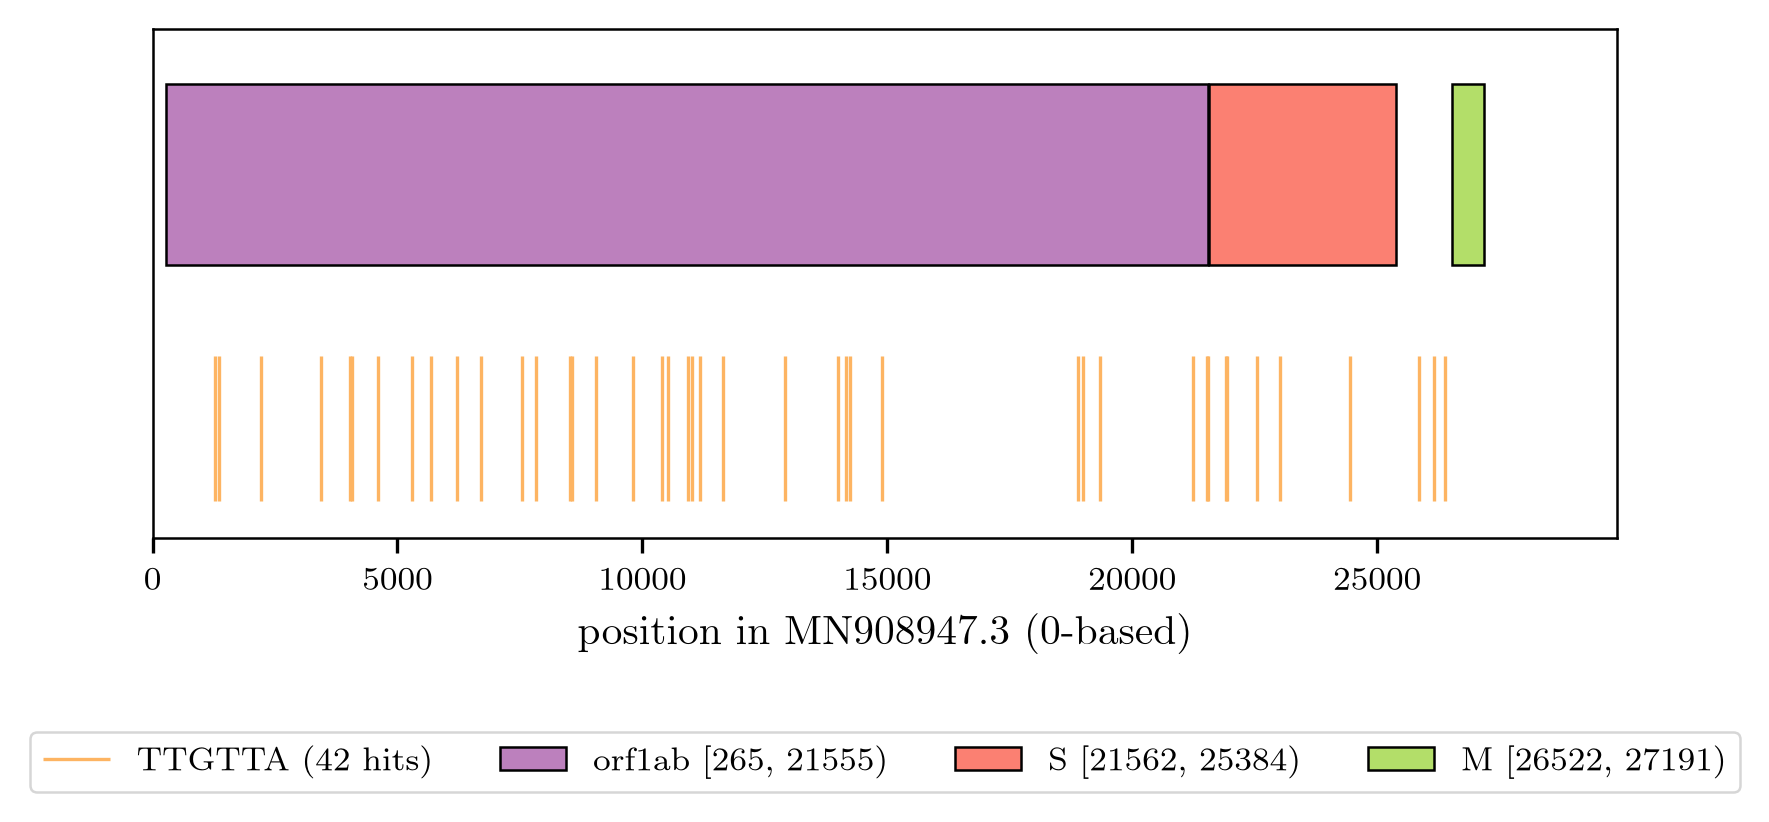
\includegraphics[width=0.85\textwidth]{fig_gene_map}
    \caption{Genes located by pattern search in the Wuhan genome and the occurrences of the most frequent 6-mer.}
    \label{fig:gene_map}
\end{figure}

\begin{figure}[H]
    \centering
    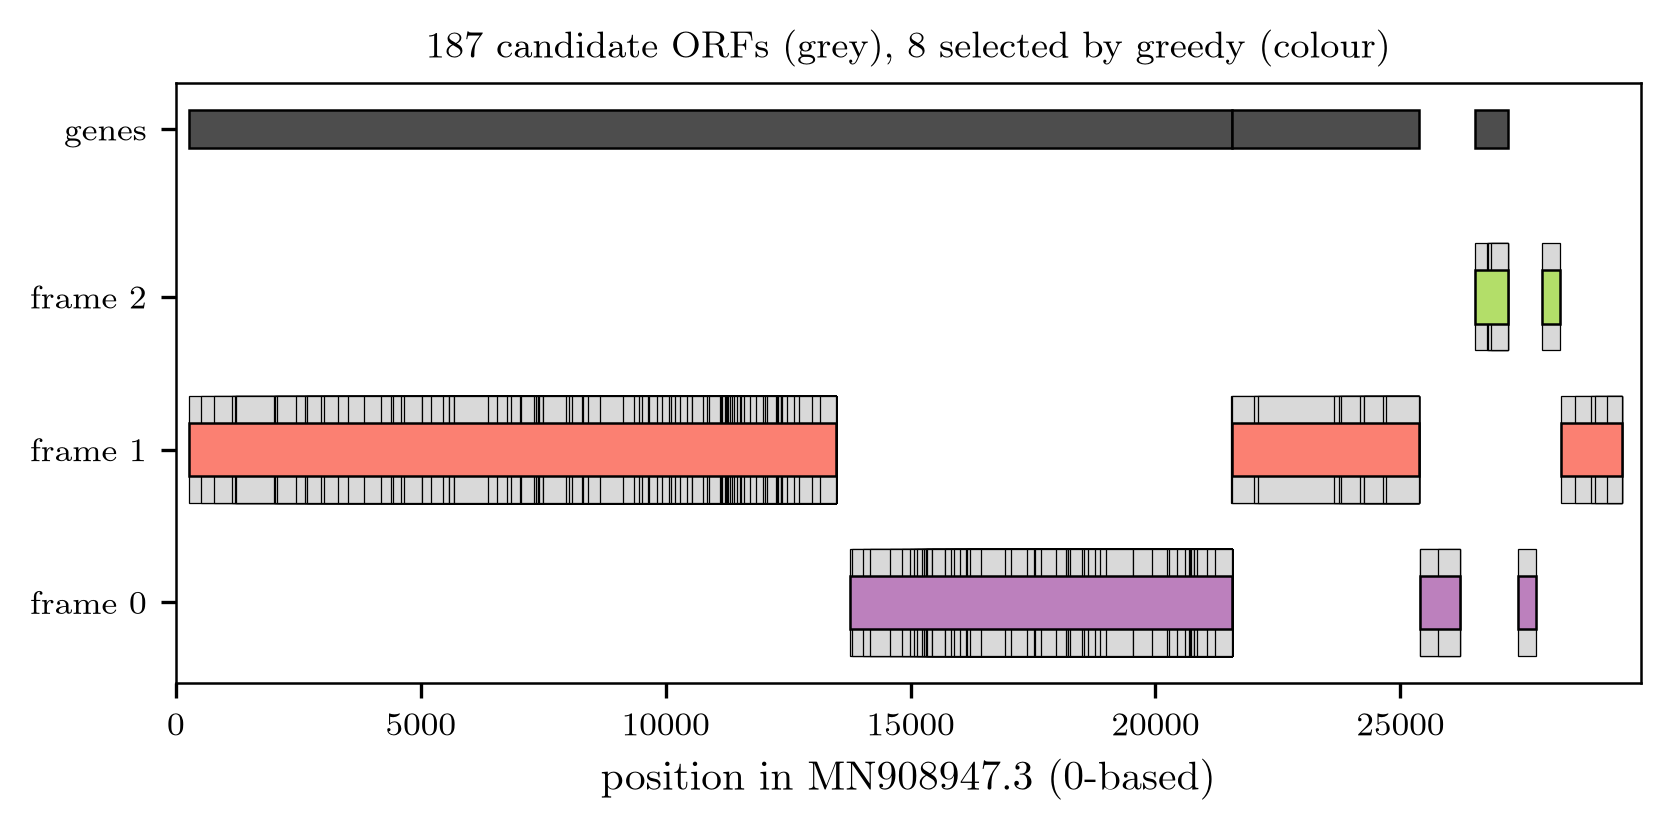
\includegraphics[width=0.85\textwidth]{fig_orf_map}
    \caption{Candidate ORFs per reading frame (grey) and the greedy selection (colour) against the known genes.}
    \label{fig:orf}
\end{figure}

\begin{figure}[H]
    \centering
    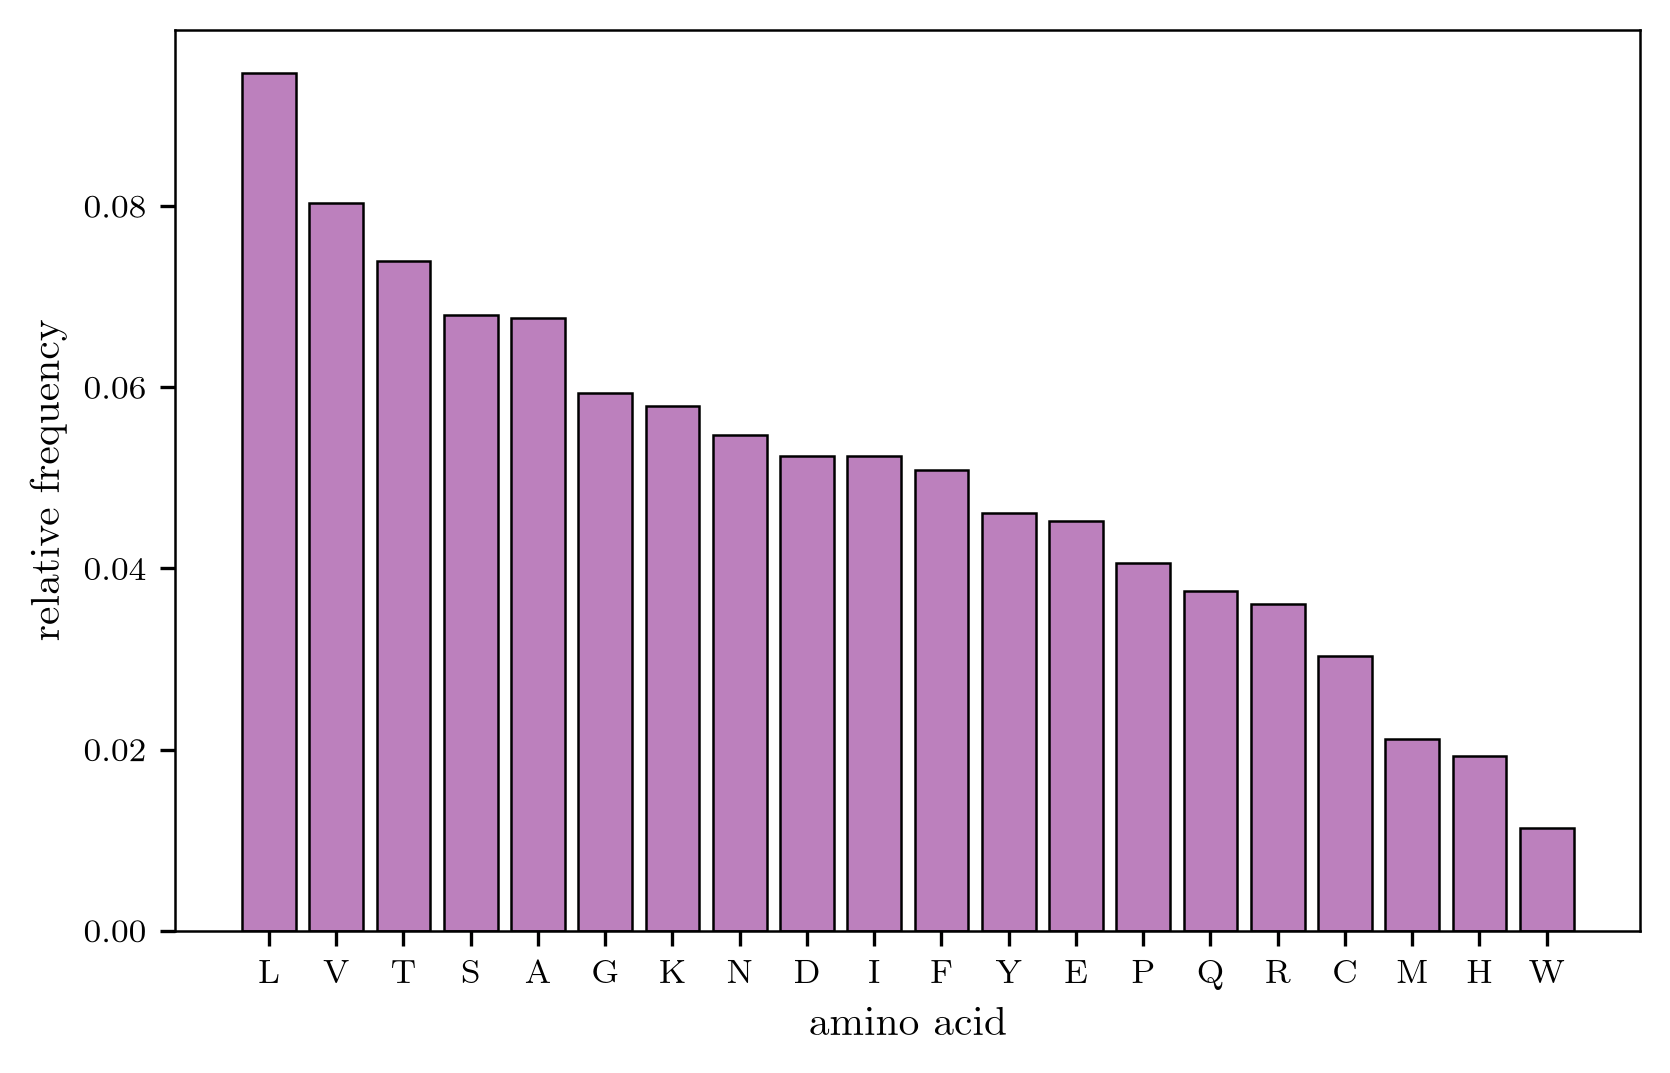
\includegraphics[width=0.7\textwidth]{fig_freq_protein}
    \caption{Pooled amino-acid frequencies over the 24 protein records.}
    \label{fig:freq_protein}
\end{figure}

\end{appendices}


\end{document}